%% CCGrid_main.tex
%% V1.3
%% 2007/01/11
%% by Michael Shell
%% See:
%% http://www.michaelshell.org/
%% for current contact information.
%%
%% This is a skeleton file demonstrating the use of IEEEtran.cls
%% (requir/Users/qybo123/Dropbox/power capping porject/paper/CCGrid2017-Yubo/abstract.texes IEEEtran.cls version 1.7 or later) with an IEEE conference paper.
%%
%% Support sites:
%% http://www.michaelshell.org/tex/ieeetran/
%% http://www.ctan.org/tex-archive/macros/latex/contrib/IEEEtran/
%% and
%% http://www.ieee.org/

%%*************************************************************************
%% Legal Notice:
%% This code is offered as-is without any warranty either expressed or
%% implied; without even the implied warranty of MERCHANTABILITY or
%% FITNESS FOR A PARTICULAR PURPOSE! 
%% User assumes all risk.
%% In no event shall IEEE or any contributor to this code be liable for
%% any damages or losses, including, but not limited to, incidental,
%% consequential, or any other damages, resulting from the use or misuse
%% of any information contained here.
%%
%% All comments are the opinions of their respective authors and are not
%% necessarily endorsed by the IEEE.
%%
%% This work is distributed under the LaTeX Project Public License (LPPL)
%% ( http://www.latex-project.org/ ) version 1.3, and may be freely used,
%% distributed and modified. A copy of the LPPL, version 1.3, is included
%% in the base LaTeX documentation of all distributions of LaTeX released
%% 2003/12/01 or later.
%% Retain all contribution notices and credits.
%% ** Modified files should be clearly indicated as such, including  **
%% ** renaming them and changing author support contact information. **
%%
%% File list of work: IEEEtran.cls, IEEEtran_HOWTO.pdf, bare_adv.tex,
%%                    bare_conf.tex, bare_jrnl.tex, bare_jrnl_compsoc.tex
%%*************************************************************************

% *** Authors should verify (and, if needed, correct) their LaTeX system  ***
% *** with the testflow diagnostic prior to trusting their LaTeX platform ***
% *** with production work. IEEE's font choices can trigger bugs that do  ***
% *** not appear when using other class files.                            ***
% The testflow support page is at:
% http://www.michaelshell.org/tex/testflow/



% Note that the a4paper option is mainly intended so that authors in
% countries using A4 can easily print to A4 and see how their papers will
% look in print - the typesetting of the document will not typically be
% affected with changes in paper size (but the bottom and side margins will).
% Use the testflow package mentioned above to verify correct handling of
% both paper sizes by the user's LaTeX system.
%
% Also note that the "draftcls" or "draftclsnofoot", not "draft", option
% should be used if it is desired that the figures are to be displayed in
% draft mode.
%
\documentclass[10pt, conference, compsocconf]{IEEEtran}
% Add the compsocconf option for Computer Society conferences.
%
% If IEEEtran.cls has not been installed into the LaTeX system files,
% manually specify the path to it like:
% \documentclass[conference]{../sty/IEEEtran}





% Some very useful LaTeX packages include:
% (uncomment the ones you want to load)


% *** MISC UTILITY PACKAGES ***
%
%\usepackage{ifpdf}
% Heiko Oberdiek's ifpdf.sty is very useful if you need conditional
% compilation based on whether the output is pdf or dvi.
% usage:
% \ifpdf
%   % pdf code
% \else
%   % dvi code
% \fi
% The latest version of ifpdf.sty can be obtained from:
% http://www.ctan.org/tex-archive/macros/latex/contrib/oberdiek/
% Also, note that IEEEtran.cls V1.7 and later provides a builtin
% \ifCLASSINFOpdf conditional that works the same way.
% When switching from latex to pdflatex and vice-versa, the compiler may
% have to be run twice to clear warning/error messages.






% *** CITATION PACKAGES ***
%
%\usepackage{cite}
% cite.sty was written by Donald Arseneau
% V1.6 and later of IEEEtran pre-defines the format of the cite.sty package
% \cite{} output to follow that of IEEE. Loading the cite package will
% result in citation numbers being automatically sorted and properly
% "compressed/ranged". e.g., [1], [9], [2], [7], [5], [6] without using
% cite.sty will become [1], [2], [5]--[7], [9] using cite.sty. cite.sty's
% \cite will automatically add leading space, if needed. Use cite.sty's
% noadjust option (cite.sty V3.8 and later) if you want to turn this off.
% cite.sty is already installed on most LaTeX systems. Be sure and use
% version 4.0 (2003-05-27) and later if using hyperref.sty. cite.sty does
% not currently provide for hyperlinked citations.
% The latest version can be obtained at:
% http://www.ctan.org/tex-archive/macros/latex/contrib/cite/
% The documentation is contained in the cite.sty file itself.






% *** GRAPHICS RELATED PACKAGES ***
%
\ifCLASSINFOpdf
  % \usepackage[pdftex]{graphicx}
  % declare the path(s) where your graphic files are
  % \graphicspath{{../pdf/}{../jpeg/}}
  % and their extensions so you won't have to specify these with
  % every instance of \includegraphics
  % \DeclareGraphicsExtensions{.pdf,.jpeg,.png}
\else
  % or other class option (dvipsone, dvipdf, if not using dvips). graphicx
  % will default to the driver specified in the system graphics.cfg if no
  % driver is specified.
  % \usepackage[dvips]{graphicx}
  % declare the path(s) where your graphic files are
  % \graphicspath{{../eps/}}
  % and their extensions so you won't have to specify these with
  % every instance of \includegraphics
  % \DeclareGraphicsExtensions{.eps}
\fi
% graphicx was written by David Carlisle and Sebastian Rahtz. It is
% required if you want graphics, photos, etc. graphicx.sty is already
% installed on most LaTeX systems. The latest version and documentation can
% be obtained at: 
% http://www.ctan.org/tex-archive/macros/latex/required/graphics/
% Another good source of documentation is "Using Imported Graphics in
% LaTeX2e" by Keith Reckdahl which can be found as epslatex.ps or
% epslatex.pdf at: http://www.ctan.org/tex-archive/info/
%
% latex, and pdflatex in dvi mode, support graphics in encapsulated
% postscript (.eps) format. pdflatex in pdf mode supports graphics
% in .pdf, .jpeg, .png and .mps (metapost) formats. Users should ensure
% that all non-photo figures use a vector format (.eps, .pdf, .mps) and
% not a bitmapped formats (.jpeg, .png). IEEE frowns on bitmapped formats
% which can result in "jaggedy"/blurry rendering of lines and letters as
% well as large increases in file sizes.
%
% You can find documentation about the pdfTeX application at:
% http://www.tug.org/applications/pdftex





% *** MATH PACKAGES ***
%
%\usepackage[cmex10]{amsmath}
% A popular package from the American Mathematical Society that provides
% many useful and powerful commands for dealing with mathematics. If using
% it, be sure to load this package with the cmex10 option to ensure that
% only type 1 fonts will utilized at all point sizes. Without this option,
% it is possible that some math symbols, particularly those within
% footnotes, will be rendered in bitmap form which will result in a
% document that can not be IEEE Xplore compliant!
%
% Also, note that the amsmath package sets \interdisplaylinepenalty to 10000
% thus preventing page breaks from occurring within multiline equations. Use:
%\interdisplaylinepenalty=2500
% after loading amsmath to restore such page breaks as IEEEtran.cls normally
% does. amsmath.sty is already installed on most LaTeX systems. The latest
% version and documentation can be obtained at:
% http://www.ctan.org/tex-archive/macros/latex/required/amslatex/math/





% *** SPECIALIZED LIST PACKAGES ***
%
%\usepackage{algorithmic}
% algorithmic.sty was written by Peter Williams and Rogerio Brito.
% This package provides an algorithmic environment fo describing algorithms.
% You can use the algorithmic environment in-text or within a figure
% environment to provide for a floating algorithm. Do NOT use the algorithm
% floating environment provided by algorithm.sty (by the same authors) or
% algorithm2e.sty (by Christophe Fiorio) as IEEE does not use dedicated
% algorithm float types and packages that provide these will not provide
% correct IEEE style captions. The latest version and documentation of
% algorithmic.sty can be obtained at:
% http://www.ctan.org/tex-archive/macros/latex/contrib/algorithms/
% There is also a support site at:
% http://algorithms.berlios.de/index.html
% Also of interest may be the (relatively newer and more customizable)
% algorithmicx.sty package by Szasz Janos:
% http://www.ctan.org/tex-archive/macros/latex/contrib/algorithmicx/




% *** ALIGNMENT PACKAGES ***
%
%\usepackage{array}
% Frank Mittelbach's and David Carlisle's array.sty patches and improves
% the standard LaTeX2e array and tabular environments to provide better
% appearance and additional user controls. As the default LaTeX2e table
% generation code is lacking to the point of almost being broken with
% respect to the quality of the end results, all users are strongly
% advised to use an enhanced (at the very least that provided by array.sty)
% set of table tools. array.sty is already installed on most systems. The
% latest version and documentation can be obtained at:
% http://www.ctan.org/tex-archive/macros/latex/required/tools/


%\usepackage{mdwmath}
%\usepackage{mdwtab}
% Also highly recommended is Mark Wooding's extremely powerful MDW tools,
% especially mdwmath.sty and mdwtab.sty which are used to format equations
% and tables, respectively. The MDWtools set is already installed on most
% LaTeX systems. The lastest version and documentation is available at:
% http://www.ctan.org/tex-archive/macros/latex/contrib/mdwtools/


% IEEEtran contains the IEEEeqnarray family of commands that can be used to
% generate multiline equations as well as matrices, tables, etc., of high
% quality.


%\usepackage{eqparbox}
% Also of notable interest is Scott Pakin's eqparbox package for creating
% (automatically sized) equal width boxes - aka "natural width parboxes".
% Available at:
% http://www.ctan.org/tex-archive/macros/latex/contrib/eqparbox/





% *** SUBFIGURE PACKAGES ***
%\usepackage[tight,footnotesize]{subfigure}
% subfigure.sty was written by Steven Douglas Cochran. This package makes it
% easy to put subfigures in your figures. e.g., "Figure 1a and 1b". For IEEE
% work, it is a good idea to load it with the tight package option to reduce
% the amount of white space around the subfigures. subfigure.sty is already
% installed on most LaTeX systems. The latest version and documentation can
% be obtained at:
% http://www.ctan.org/tex-archive/obsolete/macros/latex/contrib/subfigure/
% subfigure.sty has been superceeded by subfig.sty.



%\usepackage[caption=false]{caption}
%\usepackage[font=footnotesize]{subfig}
% subfig.sty, also written by Steven Douglas Cochran, is the modern
% replacement for subfigure.sty. However, subfig.sty requires and
% automatically loads Axel Sommerfeldt's caption.sty which will override
% IEEEtran.cls handling of captions and this will result in nonIEEE style
% figure/table captions. To prevent this problem, be sure and preload
% caption.sty with its "caption=false" package option. This is will preserve
% IEEEtran.cls handing of captions. Version 1.3 (2005/06/28) and later 
% (recommended due to many improvements over 1.2) of subfig.sty supports
% the caption=false option directly:
%\usepackage[caption=false,font=footnotesize]{subfig}
%
% The latest version and documentation can be obtained at:
% http://www.ctan.org/tex-archive/macros/latex/contrib/subfig/
% The latest version and documentation of caption.sty can be obtained at:
% http://www.ctan.org/tex-archive/macros/latex/contrib/caption/




% *** FLOAT PACKAGES ***
%
%\usepackage{fixltx2e}
% fixltx2e, the successor to the earlier fix2col.sty, was written by
% Frank Mittelbach and David Carlisle. This package corrects a few problems
% in the LaTeX2e kernel, the most notable of which is that in current
% LaTeX2e releases, the ordering of single and double column floats is not
% guaranteed to be preserved. Thus, an unpatched LaTeX2e can allow a
% single column figure to be placed prior to an earlier double column
% figure. The latest version and documentation can be found at:
% http://www.ctan.org/tex-archive/macros/latex/base/



%\usepackage{stfloats}
% stfloats.sty was written by Sigitas Tolusis. This package gives LaTeX2e
% the ability to do double column floats at the bottom of the page as well
% as the top. (e.g., "\begin{figure*}[!b]" is not normally possible in
% LaTeX2e). It also provides a command:
%\fnbelowfloat
% to enable the placement of footnotes below bottom floats (the standard
% LaTeX2e kernel puts them above bottom floats). This is an invasive package
% which rewrites many portions of the LaTeX2e float routines. It may not work
% with other packages that modify the LaTeX2e float routines. The latest
% version and documentation can be obtained at:
% http://www.ctan.org/tex-archive/macros/latex/contrib/sttools/
% Documentation is contained in the stfloats.sty comments as well as in the
% presfull.pdf file. Do not use the stfloats baselinefloat ability as IEEE
% does not allow \baselineskip to stretch. Authors submitting work to the
% IEEE should note that IEEE rarely uses double column equations and
% that authors should try to avoid such use. Do not be tempted to use the
% cuted.sty or midfloat.sty packages (also by Sigitas Tolusis) as IEEE does
% not format its papers in such ways.





% *** PDF, URL AND HYPERLINK PACKAGES ***
%
%\usepackage{url}
% url.sty was written by Donald Arseneau. It provides better support for
% handling and breaking URLs. url.sty is already installed on most LaTeX
% systems. The latest version can be obtained at:
% http://www.ctan.org/tex-archive/macros/latex/contrib/misc/
% Read the url.sty source comments for usage information. Basically,
% \url{my_url_here}.





% *** Do not adjust lengths that control margins, column widths, etc. ***
% *** Do not use packages that alter fonts (such as pslatex).         ***
% There should be no need to do such things with IEEEtran.cls V1.6 and later.
% (Unless specifically asked to do so by the journal or conference you plan
% to submit to, of course. )


% correct bad hyphenation here
\hyphenation{op-tical net-works semi-conduc-tor}


\usepackage{graphicx}
% \usepackage{enumerate}
\usepackage{amsmath}

\usepackage{subcaption}
\usepackage{tikz}
\usepackage{longtable}
\usepackage[english]{babel}
\usepackage{setspace}
%\usepackage{algorithm}
%\usepackage[noend]{algpseudocode}
%\usepackage{changepage}
\usepackage{amssymb}

% \usepackage{tabulary}

\usepackage{listings}
\usepackage{float}
\usepackage{cite}



\begin{document}
%
% paper title
% can use linebreaks \\ within to get better formatting as desired
\title{Exploring Power-Performance-Quality trade-offs for Exascale Combustion Simulation}


% author names and affiliations
% use a multiple column layout for up to two different
% affiliations

\author{\IEEEauthorblockN{Authors Name/s per 1st Affiliation (Author)}
\IEEEauthorblockA{line 1 (of Affiliation): dept. name of organization\\
line 2: name of organization, acronyms acceptable\\
line 3: City, Country\\
line 4: Email: name@xyz.com}
\and
\IEEEauthorblockN{Authors Name/s per 2nd Affiliation (Author)}
\IEEEauthorblockA{line 1 (of Affiliation): dept. name of organization\\
line 2: name of organization, acronyms acceptable\\
line 3: City, Country\\
line 4: Email: name@xyz.com}
}

% conference papers do not typically use \thanks and this command
% is locked out in conference mode. If really needed, such as for
% the acknowledgment of grants, issue a \IEEEoverridecommandlockouts
% after \documentclass

% for over three affiliations, or if they all won't fit within the width
% of the page, use this alternative format:
% 
%\author{\IEEEauthorblockN{Michael Shell\IEEEauthorrefmark{1},
%Homer Simpson\IEEEauthorrefmark{2},
%James Kirk\IEEEauthorrefmark{3}, 
%Montgomery Scott\IEEEauthorrefmark{3} and
%Eldon Tyrell\IEEEauthorrefmark{4}}
%\IEEEauthorblockA{\IEEEauthorrefmark{1}School of Electrical and Computer Engineering\\
%Georgia Institute of Technology,
%Atlanta, Georgia 30332--0250\\ Email: see http://www.michaelshell.org/contact.html}
%\IEEEauthorblockA{\IEEEauthorrefmark{2}Twentieth Century Fox, Springfield, USA\\
%Email: homer@thesimpsons.com}
%\IEEEauthorblockA{\IEEEauthorrefmark{3}Starfleet Academy, San Francisco, California 96678-2391\\
%Telephone: (800) 555--1212, Fax: (888) 555--1212}
%\IEEEauthorblockA{\IEEEauthorrefmark{4}Tyrell Inc., 123 Replicant Street, Los Angeles, California 90210--4321}}




% use for special paper notices
%\IEEEspecialpapernotice{(Invited Paper)}




% make the title area
\maketitle



\begin{abstract}
The computational demand of high-performance computing (HPC) applications has brought major changes to the HPC system architecture. As a result, it is now possible to run simulations faster and get more accurate results. But behind this, power and energy are becoming critical concerns for HPC systems, e.g. Tianhe-2 has reached speed 33.86 PFLOPS at power of 17.6 MW\cite{wiki_tianhe}, which cost electric around 30 million per year\cite{2014tianhe}. U.S. Department of Energy (DOE) has set the goal to achieve exascale performance with a power budget of 20MW\cite{lucas2014doe}, this make power efficiency become one of the critical challenges for the exascale research.

Current research efforts have studied power and performance tradeoffs, and how to balance these, e.g., using DVFS to meet power constraints, which significantly impacts performance. However, scientific applications may not tolerate degradation in performance and other tradeoffs need to be explored to meet power budgets, e.g., involving the application in making energy-performance tradeoff decisions. 

This research focuses on studying the properties and exploring the performance and power\textbackslash energy tradeoffs of Adaptive Mesh Refinement (AMR) based simulation applications. Our experimental evaluation provides an empirical evaluation of different application configurations that gives insights into the power-performance tradeoffs space for those AMR applications. The key contribution of this work is a better understanding of the running behavior of these AMR-based applications and the power-performance tradeoffs for these applications under power constraints, which can be used to better schedule power budgets across HPC systems.\cite{david2010rapl}



\end{abstract}

\begin{IEEEkeywords}
AMR; Energy; Performance; Quality; Power scheduling;

\end{IEEEkeywords}

% For peer review papers, you can put extra information on the cover
% page as needed:
% \ifCLASSOPTIONpeerreview
% \begin{center} \bfseries EDICS Category: 3-BBND \end{center}
% \fi
%
% For peerreview papers, this IEEEtran command inserts a page break and
% creates the second title. It will be ignored for other modes.
\IEEEpeerreviewmaketitle



\section{Introduction}
\label{Section:introduction}

High performance computing (HPC) has been played an important role in the field of computational science. From design perspective, HPC were built to maximize performance while irrespective of power and energy consumption, though their energy consumption has already occupied a large part of cost (i.e., operation cost). However, as we are approaching the exascale era, power is turning from an optimization goal to a critical operation constraint. U.S Department of Energy (DOE) has currently set a bound of 20MW for an exascale system.\cite{tolentino2012optimist} This strict power constraint poses a hard research challenge with current hardware and software. Sunway TaihuLight, the top one supercomputer as of June 2016, has a peak performance of 93.0 PetaFLOPS at 15.4 MW, which is 6.04 GigaFLOPS per watt. Sunway's power efficiency has improved three times then Tianhe-2. However, achieving the goal of exascale computing at 20 MW, it requires 50 GigaFLOPS per watt. So that, current HPC system still need at least a 8 times power efficiency improvement towards exascale. 

In order to achieve this exascale system power constraint, current research efforts have studied power and performance tradeoffs, and how to balance these.\cite{ge2007cpu,hsu2005power,huang2009energy,freeh2005using,donofrio2009energy,gamell2013exploring} Many power management strategies have been proposed\cite{rountree2009adagio,lim2006adaptive,ioannou2011phase,li2010hybrid,rodero2010investigating}, but most of the works are tend to choose a performance and then constraint the power consumption under that performance loss. Even if this can meet power constraints, it significantly impacts performance. In fact, most scientific applications may not tolerate degradation in performance, other tradeoffs need to be explored to meet power budgets. 





Many research efforts have studied power and performance tradeoffs, and most energy models or strategies are based on runtime (e.g., leveraging MPI slack) for power clamping or power capping techniques, like Dynamic Voltage and Frequency Scaling (DVFS) to constraint the power. However, power and performance are in the two sides of a balance scale, that it is hard to improve one side without scarifying the other one. Therefore, one of the key problems addressed in this research is keeping the power bound (or budget) without losing performance, which is challenging for real world applications targeting exascale. At the same time, it is clear that future HPC system's whole-system power constraint that will be filtered down to job-level power constrainti.e., power budgets need to be managed at application or workflow level. This indicates, as well as we believe that the applications should be involved in making tradeoffs decisions. 

This work targeting on AMR-based simulation applications. AMR method considers a hierarchy of grids of differing resolutions ranging from the coarsest to the finest. It can focus computational resources in regions of interest while decrease computing resolution in regions with less interest. Less resolution means lighter workload and less power consumption. Therefore, this flexible resolution property gives us a potential opportunity to extract power budget for other usage. In order to take best advantage of it, this work first studies the mechanisms and policies to control AMR properties, and then, it characterizes LMC power performance running on different number of cores with different levels of resolution (e.g., levels of refinement in AMR). Finally, the characterization is complemented with power capping techniques (i.e., RAPL). The overarching goal of this work is to understand the tradeoffs between power-performance and quality, and building models taking into account AMR properties for managing power budgets and workflow at scale.

The contributions of this work are summarized below:
\begin{enumerate}
\item It presents an empirical evaluation of different configurations of application that gives insights into the energy-performance-quality tradeoffs for scientific data-driven workflows. 
\item It provides a comprehensive study of this LMC simulation performance, quality, and power and energy behavior.
\item It presents a proof-of-concept study of potential of power capping and power management to balance power-performance-quality tradeoffs.
\end{enumerate}


The rest of this thesis is organized as follows. Section \ref{Section:related work} summarizes the related work. Section \ref{Section:approach} presents the proof of concepts. Section \ref{Section:experiments} describes the evaluation methodology and presents the results of the experimental evaluation. Section \ref{Section:conclution} concludes the chapter and outlines ongoing and future research.




\section{Related works}
\label{Section:related work}

Energy efficiency has become a critical concern for HPC applications. Many algorithms, energy models and run-time systems have been proposed and developed to obtain energy saving during HPC application execution. DVFS and CPU throttling operations are two practical power saving methods. By leveraging those two methods, Kandalla et al. \cite{kandalla2010designing} designed power-aware algorithms that deliver fine-grained power savings the communication phases of single parallel programming model, typically MPI. At meantime, Li et al. \cite{li2010hybrid} extended this power-aware performance prediction model to hybrid MPI/OpenMP applications which can achieve better energy-efficient execution. In addition, in system level, Rountree et al. \cite{rodero2010investigating} developed a runtime system called Adagio, by doing the critical path analysis, it can determine which tasks may be slowed down and also suitable opportunities to apply DVFS to minimize the performance loss in the parallel execution. Ioannou et al. \cite{ioannou2011phase}  describe a runtime system for the Intel Single-chip Cloud Computer (SCC) processor to detect repeatable communication phases followed by an application of frequency scaling. 

In addition to those power saving work, there also have lots of research works on investigating power management. Lively et al. \cite{lively2011energy}  explored and investigated energy consumption and execution time of MPI only versus hybrid MPI/OpenMP parallel implementations of scientific applications on HPC systems. Gamell et al. \cite{gamell2013exploring} used machine independent code characteristics to build a power model and leverage it to analyze the behavior of simulation workflows and explore data-related energy / performance trade-offs at extreme scales. Rodero et al. \cite{rodero2010investigating} studied the potential of application-centric aggressive power management of HPC scientific workloads and leverage several innovative approaches to tackle the problems in power management mechanisms and controls available at different levels and different subsystems. Power budget could be potentially wasted in processors imbalance usage. A peak power management technique for multi-core systems has been described by Sartori et al cite{sartori2009distributed} , that through choosing the power state for each core to meet the power constraints. Also, several researches study the power budget arrangement. Cebrian et al. \cite{cebrian2011power} proposed that through borrowing power budgets from cores that consume lower power to dynamically adapts the per-core power budgets. While, Gandhi et al. \cite{gandhi2009power} give a power capping strategy to meet the power budget by inserting idle cycles during execution. Moreover, power budget can be constrained by dynamic reconfiguring processors? resources, such as Meng et al. \cite{meng2008multi} proposed to dynamic resizing cache and Konotorinis et al. \cite{kontorinis2009reducing} proposed to reconfigure load-store queues n floating point units and, etc. 

Most of above power management strategies are using DVFS. Since Intel SandyBridge family processors, Intel provides Running Average Power Limit (RAPL) for controlling the power constraint on processors and memory. Several studies have evaluated the RAPL power management system. Zhang et al. \cite{zhang2015quantitative} give a systematic evaluation of RAPL behavior such as stability, setting time, overshoot and, etc. Rountree et al. \cite{rountree2012beyond} through evaluated power consumption for package and memory subsystem to explore RAPL as a replacement for DVFS in HPC systems. In \cite{porterfield2015application}\cite{sarood2013optimizing}, RAPL also been used to study application runtime variability and power optimization for exascale computing.
Measuring the power/energy consumption is the key for energy-aware scheduling. RAPL provides power measurement ability which mechanism and performance have been investigated in \cite{porterfield2015application} \cite{hahnel2012measuring}. Vignesh et al. \cite{adhinarayanan2015greenness} use RAPL to measure the CPUs and RAMs power consumption, in order to study the greenness of the in-situ and the post-processing visualization pipelines and claim that the average RAPL measurement error rate of less than 1\%. 












\section{POWER SCHEDULING FOR AMR WORKLOADS}
\label{Section:approach}
In this work, we are trying to explore the trade-offs among  power, performance and quality of exascale simulation applications.  These simulation applications are based on Adaptive Mesh Refinement (AMR) method, which  is a method of dynamically adapting the solution's resolution within certain region of simulation. In 1984, Berger and Oliger proposed using AMR for computing time-dependent solutions to hyperbolic partial differential equations in multiple space dimensions. \cite{berger1984adaptive} Later on, they and Phillip Colella developed local adaptive mesh refinement algorithm for dynamic gridding.\cite{berger1989local} And since then, this AMR approach has been used in solving or simulating a variety engineering problems.\cite{berger1984adaptive,powell1993adaptive,bell1994three} The beauty of AMR is that it only focus computational resources in regions of interest but decrease solution's resolution in regions with less interest. By doing this, it largely increases computational utilization and therefore minimizes memory and storage requirements. It is powerful especially in solving problems with multiple scales. 

AMR algorithm uses a hierarchical grid structure, which typically is composed of rectangular in various sizes. The basic adaptive refinement strategy is to refine on logically rectangular patches. From very beginning, the entire problem domain is covered by level 0 grids. As time step moves on, some rectangular portions of level 0 grid are covered by level 1 grids which refined by refinement factor \textit{R} in each direction. Then, regions of each level 1 grid might be covered by level 2 grids, and so on. \cite{AMRalgorithms} Between each step, there is synchronization operations that insure correct behavior at the coarse-fine interfaces, and regridding operations which permit the refined grids to track complex and /or interesting regions of the flow. Therefore, as the level of refinement increase, the number of grids increase  geometrically. These simulation applications using AMR method, on the one hand will  improve computational utilization, on the other hand , the workload will largely increase as they increase solution resolution. 

At meantime, current HPC applications by default are consuming all computational resource and  typically running for relatively long time and usually under certain power budget as well. In this case, if there is a small but urgent work need to be done. How to schedule it to run? From this point of view, we want to investigate if we can create some power budget and computational resource from the current running task while not affect their performance to run other extra tasks. In order to create this power budget, there are two obvious factors we can change, the simulation resolution, and the CPU power.  

In order to explore the trade-offs, we first evaluated the relationship among AMR refinement resolution, CPU power level and the energy consumption. As shown in the Figure \ref{fig:Energy_consumption_trend}, we execute a simulation application, the execution time will increase as the level of refinement/resolution increases or cap down CPU power. The energy consumption presents the same trend as the execution time. The question here is how to use this characterization to create available power budget. We propose to combine these two factors, adjusting resolution and applying appropriate power capping, to get available power budget.

To further demonstrate this concept, we measure the LMC execution time (will replace it with another application) with different resolution levels on 64 cores, as shown in Figure \ref{fig:LMCruntime}. Obviously, the execution time is decreasing as we degrading the resolution levels. In the meantime, capping down the CPU power will increase the execution time. Therefore, if applying appropriate power capping to it, then each execution can be the same. In the work, since we define the execution time as the performance criteria, by adjusting resolution and applying appropriate power capping, we can keep the performance while having the available power budget, shown as the red shadow area in Figure \ref{fig:Available_power_budget}.
Also, by doing so, the memory pressure release a lot, by XX percentage. Since the AMR workload reduce (decrease level of refinement, will reduce the amount of grids), the I/O usage is release a lot, as well. 
























\textbf{Configuration}
\begin{table}[H]
\begin{center}
\begin{tabular}{|l|l|}
	\hline
	\textbf{Parameter} & \textbf{Value}\\ \hline
    Platform & CAPER cluster\\ 		\hline
    Number of cores & 64 cores\\
	\hline
	Resolution & level 3 2 1\\
    \hline
    Time step & 10\\
    \hline
    Time unit & Second\\
    \hline
    Power measurement & RAPL meter\\
    \hline
    Power cap & RAPL\\
    \hline
\end{tabular}
\end{center}
\caption{Configuration for experiment of getting available power budget through power capping and resolution degradation
}
\label{table:table_tradeoff}
\end{table}



\begin{figure}[H]
	\centering
    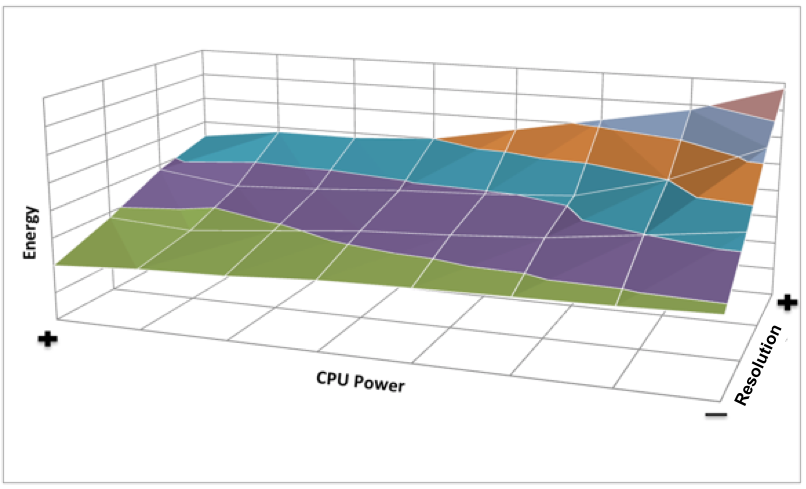
\includegraphics[width=8cm]{figs/Energy_consumption_trend.png}
        \caption{Energy consumption trend for different power caps and refinement levels}
        \label{fig:Energy_consumption_trend}
\end{figure}

\begin{figure}[H]
	\centering
    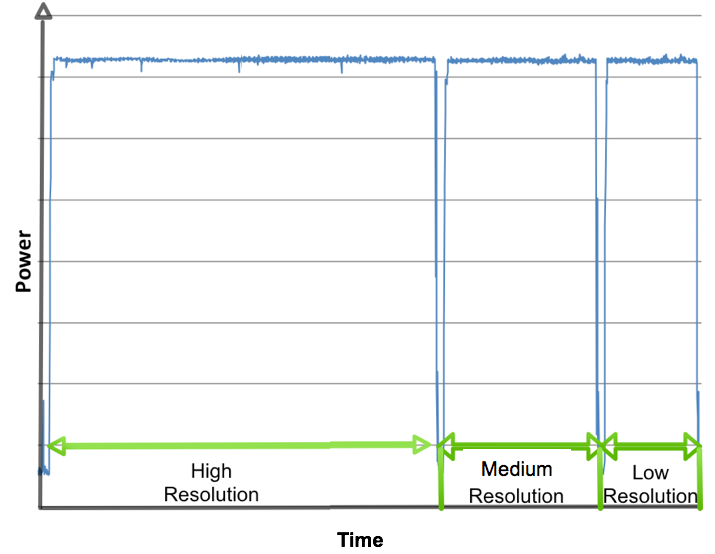
\includegraphics[width=8cm]{figs/LMCruntime.png}
        \caption{LMC power consumption curve with different (qualitative) resolution levels on 64 cores}
        \label{fig:LMCruntime}
\end{figure}


\begin{figure}[H]
	\centering
    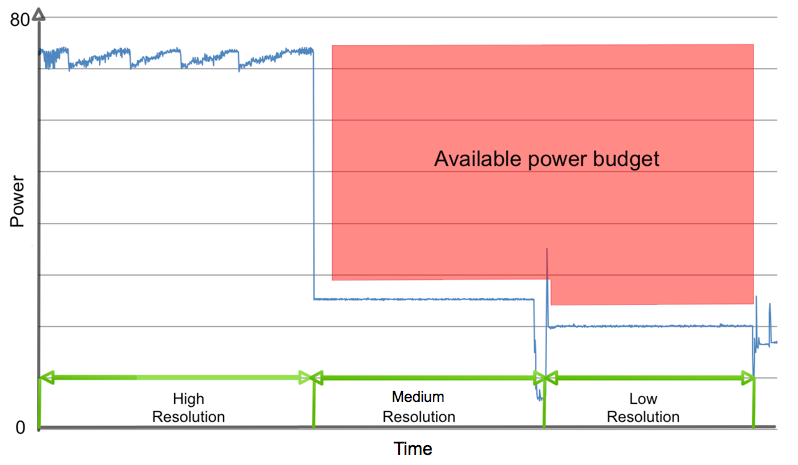
\includegraphics[width=8cm]{figs/Available_power_budget.png}
        \caption{Available power budget from applying resolution degradation and appropriate power capping}
        \label{fig:Available_power_budget}
\end{figure}






















































\section{Experimental evaluation}
\label{Section:experiments}
\subsection{Infrastructure overviews}
Caliburn
Caliburn is the new supercomputer from RDI2, which is ranked \#166 worldwide in the Top500 list of June 2016. This system is based on TatTwin SuperServer solution and it has 560 nodes containing 20,160 cores, 140 TB of RAM memory, 218 TB of non-volatile memory and 100 Gbps Omni-Path fabric (OPA) interconnection, which deliver performance of 603 TFLOPS with a peak performance of 677 TFLOPS.  Other details of each node's hardware is given in Table \ref{table:caliburn_hardware_specification}.

\begin{table}[H]
\begin{center}
\begin{tabular}{|l|l|}
	\hline
	\textbf{H/W Type} & \textbf{H/W Detail}\\ \hline
    CPU & 2\* Intel Xeon E5-2695v4\\ 		
    \hline
    CPU frequency & 2.1 GHz\\
    \hline
    \# of Cores & 2\* 18\\
    \hline
    Cache & 2\* 45 MB\\
    \hline
    Memory &\\
    \hline
    Disk & \\
    \hline
    Network bandwidth & \\
    \hline
\end{tabular}
\caption{Caliburn hardware specification}
\label{table:caliburn_hardware_specification}
\end{center}
\end{table}



\subsection{Power measurement}
The Caliburn supports Intelligent Platform Management Interface (IPMI), which is a set of computer interface specifications that is led by Intel\cite{wikiipmi}. This IPMI provides independently management and monitoring capabilities of host system's CPU, firmware and operation system and also allow administrators to manage the system remotely and monitor platform status as well, such as system power supplies, temperatures, fans and ,etc. The Caliburn vendor Supermicro provides a tool called SMCIPMITOOL, which gives power measurement function to users via a command line interface\cite{SMCIPMITOOLuserguide}. In the current system set up, the SMCIPMITOOL can provide us concurrently system-wide total power consumption of two nodes. In this case, all of our experiments are running in even number of nodes. SMCIPMITOOL not give high sample rate, as we test, it give roughly 0.5 Hz sampling rate.  [****need to consult Koji about Caliburn IPMI setup details and SMCIPMITOOL measurement accuracy****]


\subsection{Power capping}
Intel Running Average Power Limit (RAPL) provides a standard interface for measuring and constraining processor and memory power. Based on Intel publication \cite{david2010rapl}, RAPL has combined automatic DVFS and clock throttling techniques, but unlike most popular power capping mechanisms that maintain instantaneous power limits, RAPL estimates and maintains an average power limit over a sliding time window. In some studies\cite{rountree2012beyond,sarood2013optimizing}, RAPL gives high accuracy power capping performance. In our experiment, we use Intel RAPL toolkit, call Intel Power Gadget to set power bound.


\subsection{Performance measurement}
In this study, cannot find a universal standard to quantify the impact for these simulation applications result and performance. Therefore, we propose to quantify its scientific impact from system perspective, specifically, by evaluating CPU utilization, I/O traffic, memory pressure and network traffic. To measure those type of data, we are using two profiling tools: perf and sar. 

Perf is a performance analysis tool in Linux, it offers a rich set of commands to collect and analyze performance and trace data. Sar is a Unix System monitor, it can report on various system loads, to measure memory/paging, device load and network. We use the commands listed in  \ref{table:performance properties} to profiling performance .


\begin{table}[H]
\begin{center}
\begin{tabular}{|l|l|}
	\hline
	\textbf{Property} & \textbf{Command line}\\ \hline
    CPU & perf stat -B\\ 		\hline
    I/O & sar -b\\				\hline
    Memory & sar -r\\			\hline
    Network & sar -n DEV\\      \hline
\end{tabular}
\caption{Performance properties measured and respective command lines }
\label{table:performance properties}
\end{center}
\end{table}



\subsection{Application configurations}
These four simulation applications are simulating different problems, but they all based on AMR algorithm, which uses a hierarchical grid structure, and fill finer patches on the region of interest. We tune their refinement level via their input configuration, to have high, medium and low resolutions. We adjust each application's AMR level of refinement via tuning the parameters in \ref{table:amr_resolution}.


\begin{table}[H]
\begin{center}
\begin{tabular}{|l|l|}
	\hline
	\textbf{Application name} & \textbf{AMR resolution parameter}\\ \hline
    ENZO & MaximumRefinementLevel\\ 		\hline
    FLASH & lrefine\_max\\				\hline
   RAMSES & levelmax\\			\hline
    LMC & amr.max\_level\\      \hline
\end{tabular}
\caption{AMR resolution parameters of each simulation application}
\label{table:amr_resolution}
\end{center}
\end{table}

Some applications have their own I/O libraries dependence. FLASH is using parallel version HDF5, otherwise, the I/O is only called by a single CPU. Network is through Intel Omni-path and the MPI is compiled with OpenMPI-1.10.0-hfi.



\subsection{Methodology}
\subsubsection{Finding appropriate power value, using power cap}
In the previous section, we conclude that the application execution time will decrease as level of refinement/resolution decrease or increase as capping down CPU power. In order to keep application execution time the same with high, medium and low resolution, we first record the execution time of high resolution without implement power cap, and then iteratively capping down CPU power by 10 W for running application in medium or low resolution, until their execution time is matching the high resolution?s execution time within 5\% difference. In this way, we can get the appropriate power cap value for each level of resolution.

\subsubsection{Measuring performance}
This experiment is running on 512 cores across 15 nodes. However, due to the limitation of Perf and Sar, they only can profile a single node. Therefore, we only profile the node that launch the experiment. For example, the experiment is running from node 1 to node 15, then we only measure the performance of node 1. In addition, the power consumption measurement covers all the 15 nodes. SMCIPMITOOL is running on login node, and can measure every node?s power consumption.










\section{Results}
\subsubsection{Evaluation of different levels of refinement for different number of cores}
This experiment is first run on CAPER cluster, with a maximum of 128 cores, from level 1 to level 4 on 2, 4, 8, 16, 32, 64 and 128 cores. The execution time is recorded simply with the system tool ``time''.

\noindent
\textbf{Configuration}
\begin{table}[H]
\begin{center}
\begin{tabular}{|l|l|}
	\hline
	\textbf{Parameter} & \textbf{Value}\\ \hline
    Platform & CAPER and DELL cluster\\ 		\hline
    Number of cores & 2 to 128 quadratic growth\\
	\hline
    Level of refinement  & level 1 to level 4\\
    \hline
    Time step & 10\\
    \hline
    Time unit & Second\\
    \hline
\end{tabular}
\end{center}
\caption{Configuration for experiment of execution time of different levels of refinement under variety number of cores
}
\label{table:table_time_refinement}
\end{table}


\noindent
%\textbf{Result}
\begin{figure}[H]
	\centering
    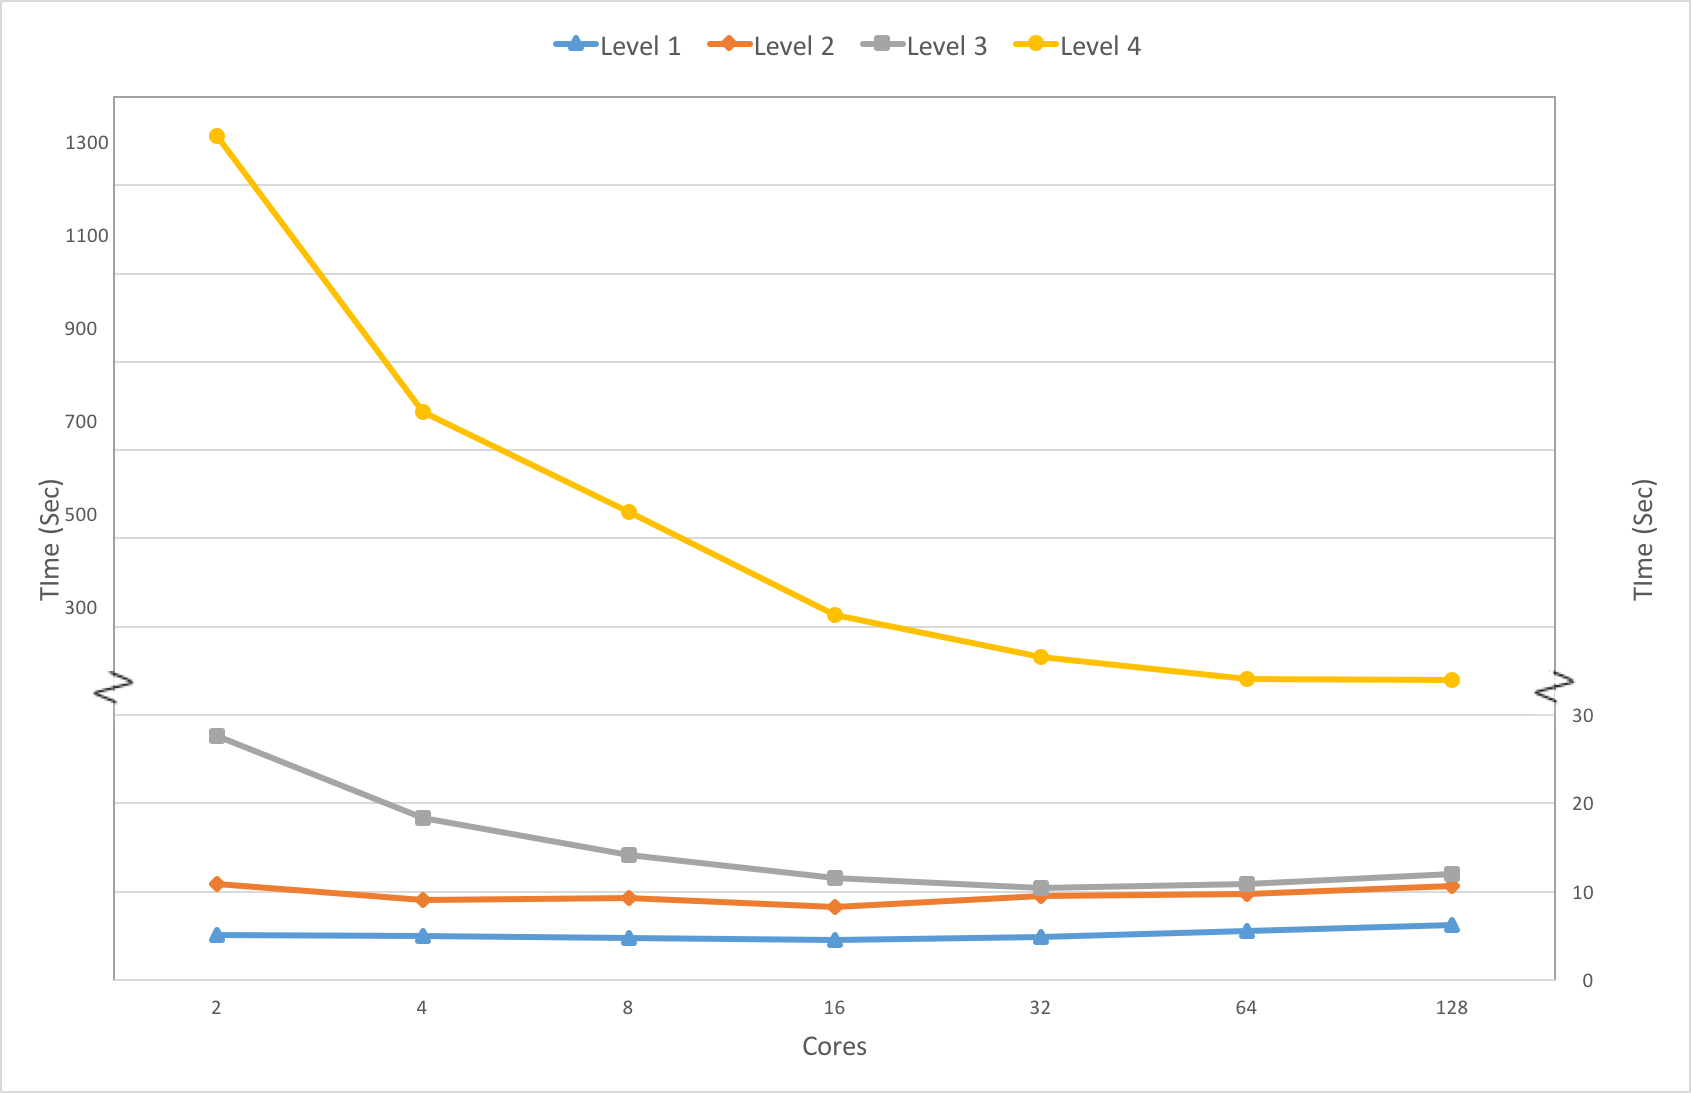
\includegraphics[width=8cm]{figs/CAPER_lev1-4_run_time_edited.jpg}
        \caption{Execution time of running different levels LMC on CAPER cluster through 2 to 128 cores. }
        \label{fig:executiontimeoncaper}
\end{figure}

\begin{figure}[H]
	\centering
    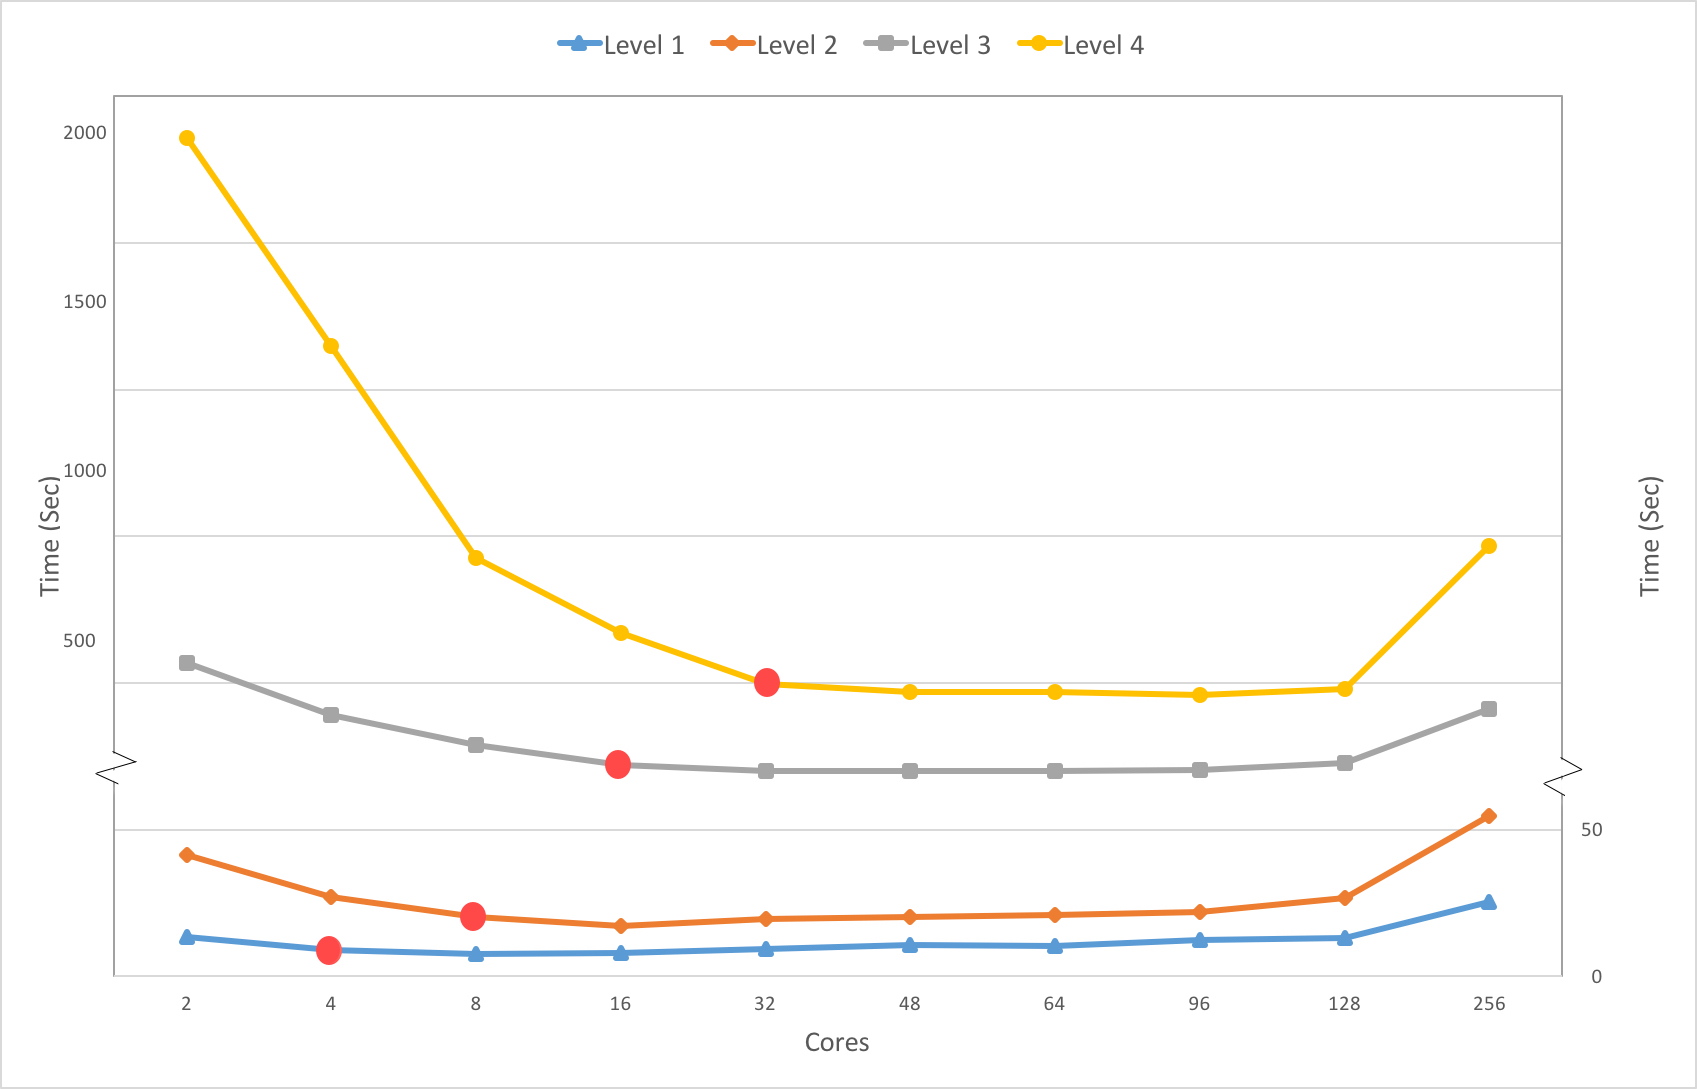
\includegraphics[width=8cm]{figs/Dell_lev1-4_run_time_edited.jpg}
        \caption{Execution time of running different levels LMC on DELL cluster through 2 to 256 cores. }
        \label{fig:executiontimeondell}
\end{figure}

%\noindent
%\textbf{Discussion}

The results of the first experiment using CAPER cluster are shown in Figure \ref{fig:executiontimeoncaper}. As can be clearly seen from the level 4 line, which is yellow line with solid dot maker, the more computing resource we use, the faster the execution is. Comparing these four lines, we can also notice that the slope is decreasing from level 4 to level 1, and then the lines go to a relative flat zoom. From this notice, we can see that heavier workload need more computational resources, but provisioning more resources do not bring any performance increase. In Figure \ref{fig:executiontimeoncaper} it can be seen from level 1 to level 3 lines that their tails are tilting a little bit, but level 4 line doesn’t have this trend. In order to show its trend more clearly, we ran this experiment on DELL cluster (256 cores cluster). The result is shown in Figure \ref{fig:executiontimeondell}. All levels' curve is like a ``U'', that tilt in the head and tile. From level 1 to level 4, the head turning point, which marked by red dot, are respectively 4, 8, 16 and 32 cores. Then they tend to get into a flat zoom, while under the 256 core, the execution time are all increase. From these two experiments we can conclude that, to achieve optimal running time, we need to configure appropriate number of processors to execute certain level of quality for the LMC program and using more processors does guarantee better performance.



\subsubsection{Evaluation of energy consumption of different levels of refinement under variety number of cores}
In this experiment, we are aim at exploring the energy consumption of running LMC with different level of refinement under multiple number of cores. 

%\noindent
%\textbf{Methodology}

Energy is the product of power and time, therefore, in this experiment, we need to measure the execution time and power respectively. To measure time, we still use Linux command TIME in the script file. And for the CPU power, we are using RAPL power meter to measure it. RAPL power meter is a sub-function of Intel Power Gadget program, which has been mentioned in previous background section. We are sampling power data every 0.5 second.

\noindent
\textbf{Configuration}
\begin{table}[H]
\begin{center}
\begin{tabular}{|l|l|}
	\hline
	\textbf{Parameter} & \textbf{Value}\\ \hline
    Platform & CAPER cluster\\ 		\hline
    Number of cores & 2 – 128 quadratic growth\\
	\hline
    Level of refinement  & level 1 to level 4\\
    \hline
    Time step & 10\\
    \hline
    Time unit & Second\\
    \hline
    Power measurement object & 8 nodes processors\\
    \hline
    RAPL sample rate & 2 Hz\\
    \hline
\end{tabular}
\end{center}
\caption{Configuration for experiment of power consumption of different levels of refinement under variety number of cores
}
\label{table:table_power_refinement}
\end{table}

\noindent
%\textbf{Result}
\begin{figure}[H]
	\centering
    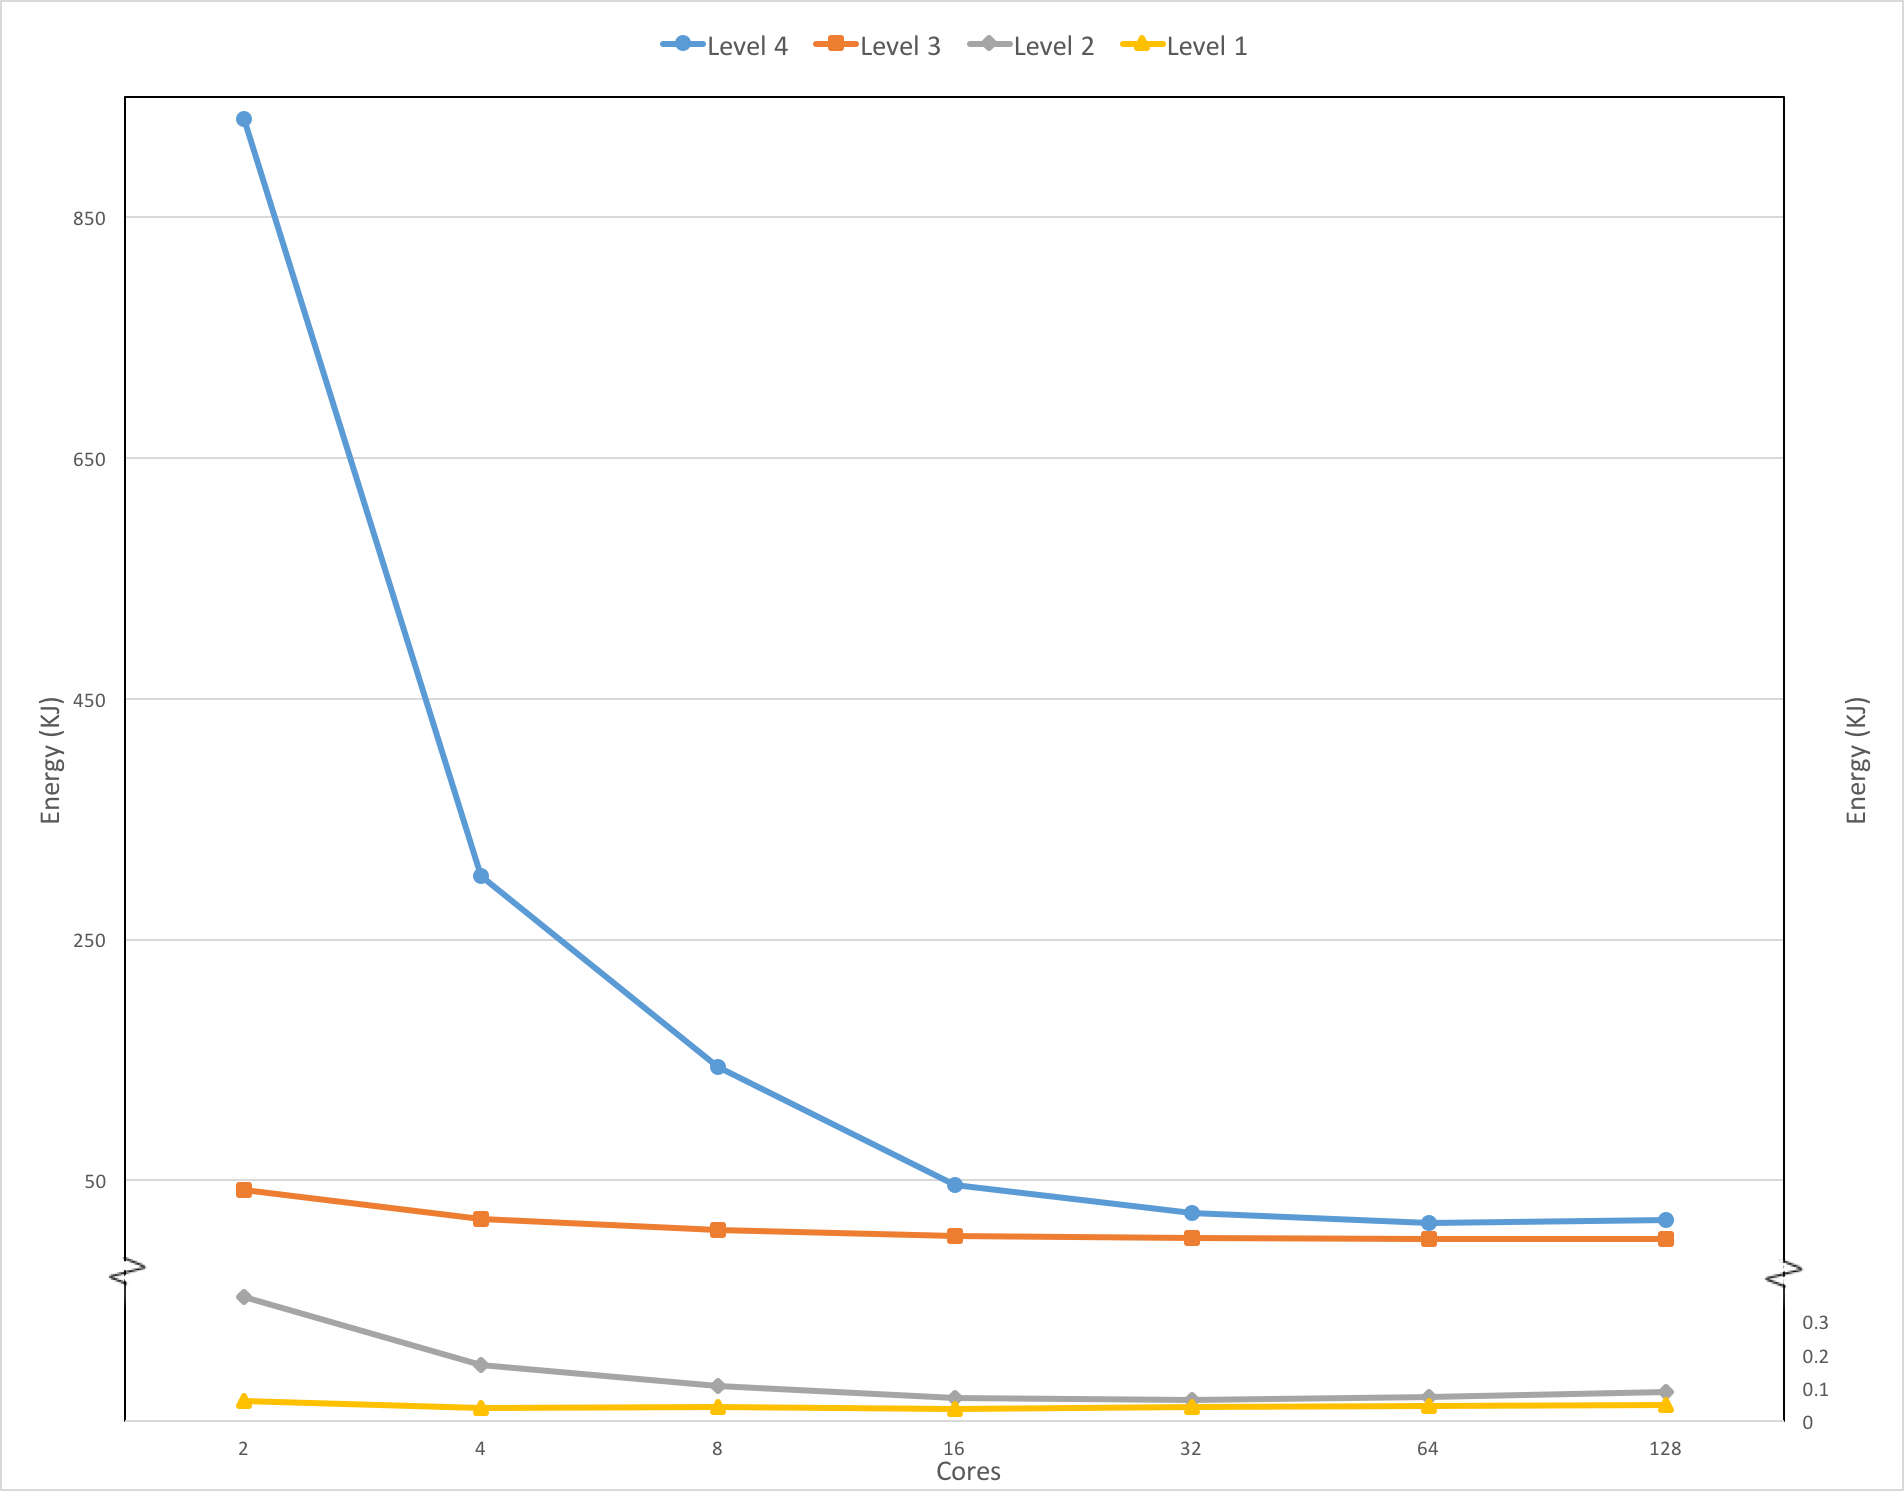
\includegraphics[width=8cm]{figs/CAPER_lev1-4_power_edited.jpg}
        \caption{Power consumption of different levels of refinement under different number of cores }
        \label{fig:powerconsumptioncaper}
\end{figure}

\noindent
%\textbf{Discussion}

Figure \ref{fig:powerconsumptioncaper} shows that there is a huge energy difference on the beginning of this curve. When running on 2 cores, the highest one (level 4) consumes almost 930 KJ while the lowest one (level 1) only take around 0.6 KJ. Since this experiment measure the all 8 node processors power status, the huge energy consumption of level 4 comes from the long execution time. It takes 1,314 seconds to run level 4 job while only 10 seconds to execute level 1. Most energy consumption comes from processors in idle state. But when assign appropriate processor resources to it, the curve reaches the flat zoom, the energy consumption difference is reasonable and stable. From this point of view, an appropriate number of cores for a certain workload is very crucial for energy consumption.



\subsubsection{Evaluation of the impact of RAPL power capping on LMC performance }
This experiment is aimed at studying the impact of power capping on LMC power-performance. And it would also give us a reference about the optimal power capping setting for different resolution levels. 


%\noindent
%\textbf{Methodology}

We use level 1 to level 4 in LMC as inputs to measure the time and power consumption. Since CAPER CPU power is 95W (Intel Xeon E5-2650 V2), in this experiment, we cap the CPU power to 25W, 35W, 45W, 55W, 65W, 75W, 85W, and 95W and record the package energy consumption (PKG) and execution time respectively. Package energy consumption is the energy used by the CPU chip itself including cores, caches and graphics, etc. 


\noindent
\textbf{Configuration}
\begin{table}[H]
\begin{center}
\begin{tabular}{|l|l|}
	\hline
	\textbf{Parameter} & \textbf{Value}\\ \hline
    Platform & CAPER cluster\\ 		\hline
    Number of cores & 64 cores\\
	\hline
    Level of refinement  & level 1 to level 4\\
    \hline
    Time step & 10\\
    \hline
    Time unit & Second\\
    \hline
    Power measurement object & 8 nodes processors\\
    \hline
    Power capping & 95W to 25W decrease by 10\\
    \hline
    RAPL sample rate & 2 Hz\\
    \hline
\end{tabular}
\end{center}
\caption{Configuration for experiment of exploring the affection of RAPL power capping on LMC performance 
}
\label{table:table_rapl_capping}
\end{table}

%\textbf{Power capping with RAPL}\\
We use Intel \textit{power\_gadget} tool to cap the power. To use it, we assign value to the parameter \textit{MY\_POWER\_LIMIT}, then compile and run it.
We use linux command line ``time'' to measure the execution time. The execution command line is provided as follows:
%\begin{adjustwidth}{2cm}{4cm}
time mpirun -machinefile hostfile.txt -np 64 .\/LMC2d.Linux.g++.gfortran.SDC.MPI.ex inputfile amr.max\_lev=\#level
%\end{adjustwidth}

For the power measurement, we also use the Intel \textit{power\_gadget} tool. When running it, it will give the real-time power consumption data every 0.5 second.



\noindent
%\textbf{Result}
\begin{figure}[H]
	\centering
    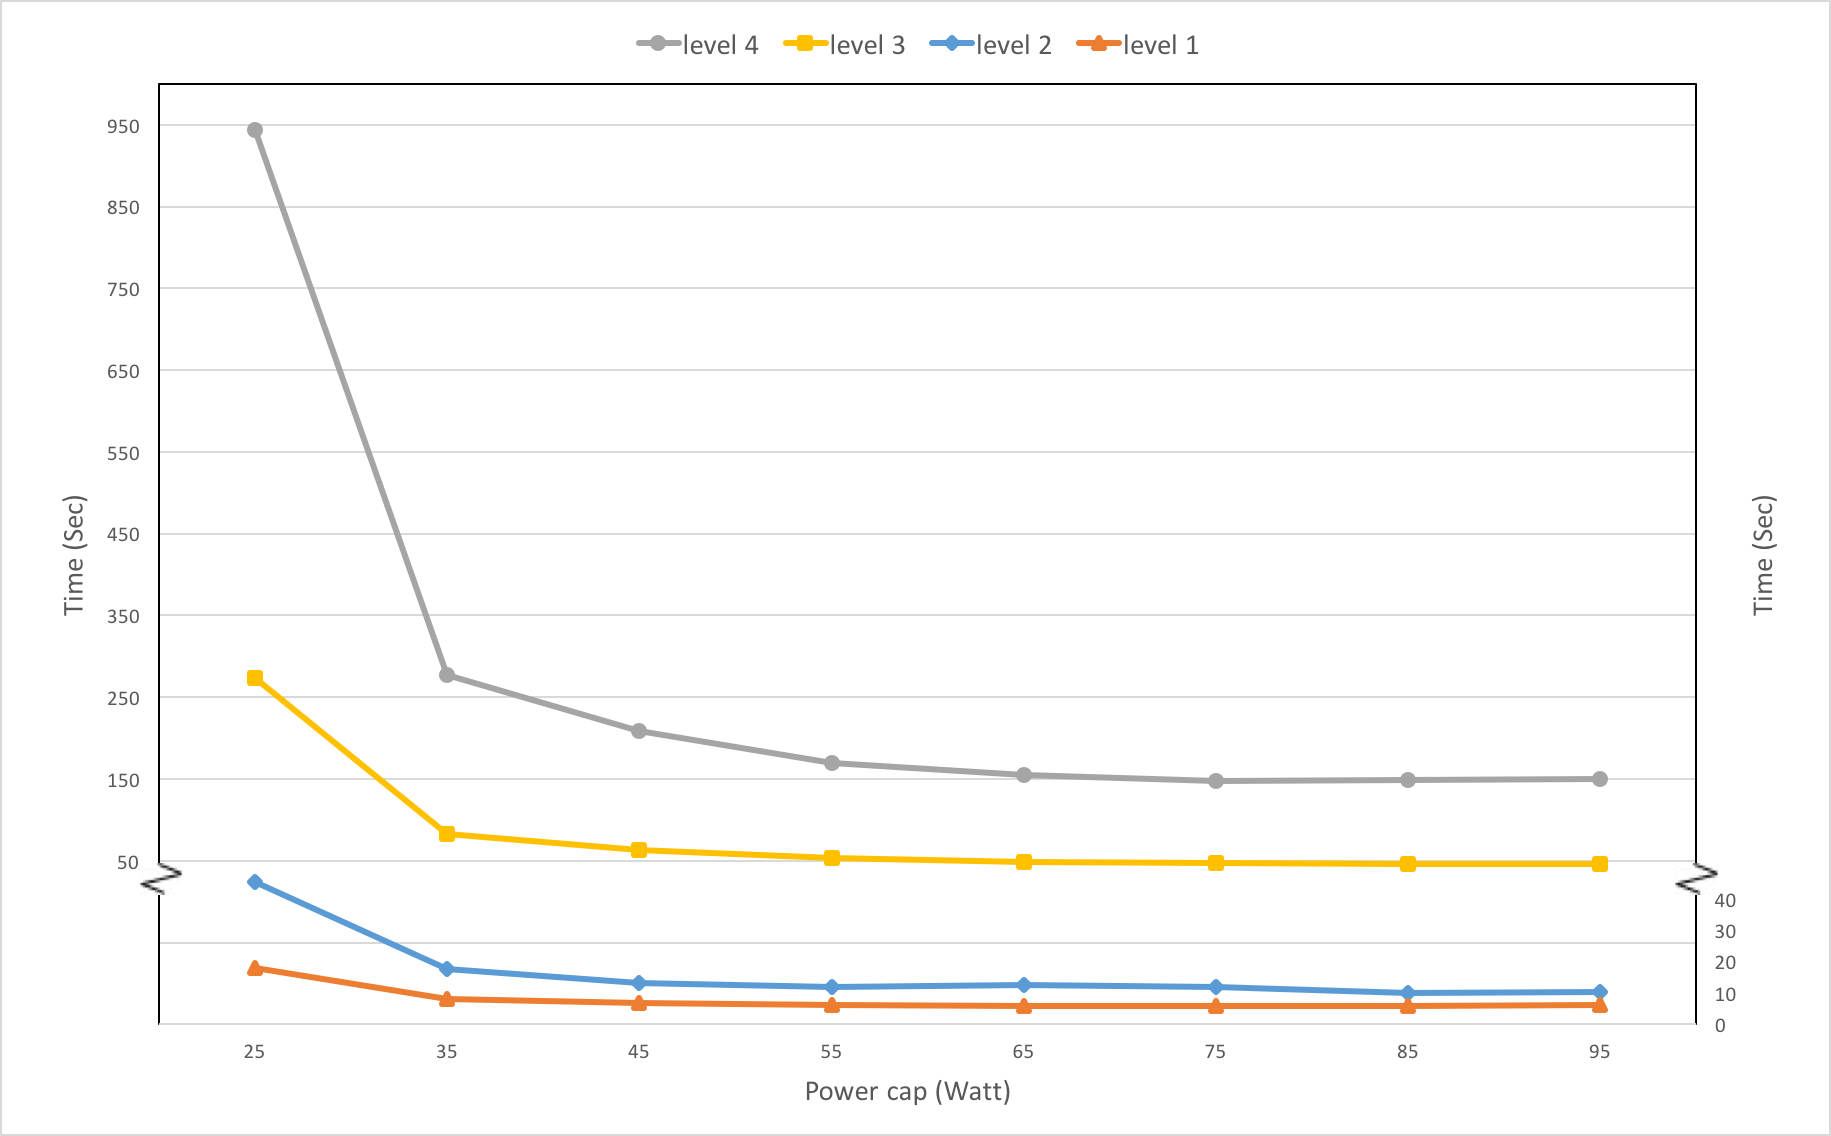
\includegraphics[width=8cm]{figs/CAPER_lev1-4_power_cap_time_edited.png}
        \caption{Relationship between different resolution of LMC and their execution time under different power capping levels}
        \label{fig:RAPLpowercaptime}
\end{figure}

\begin{figure}[H]
	\centering
    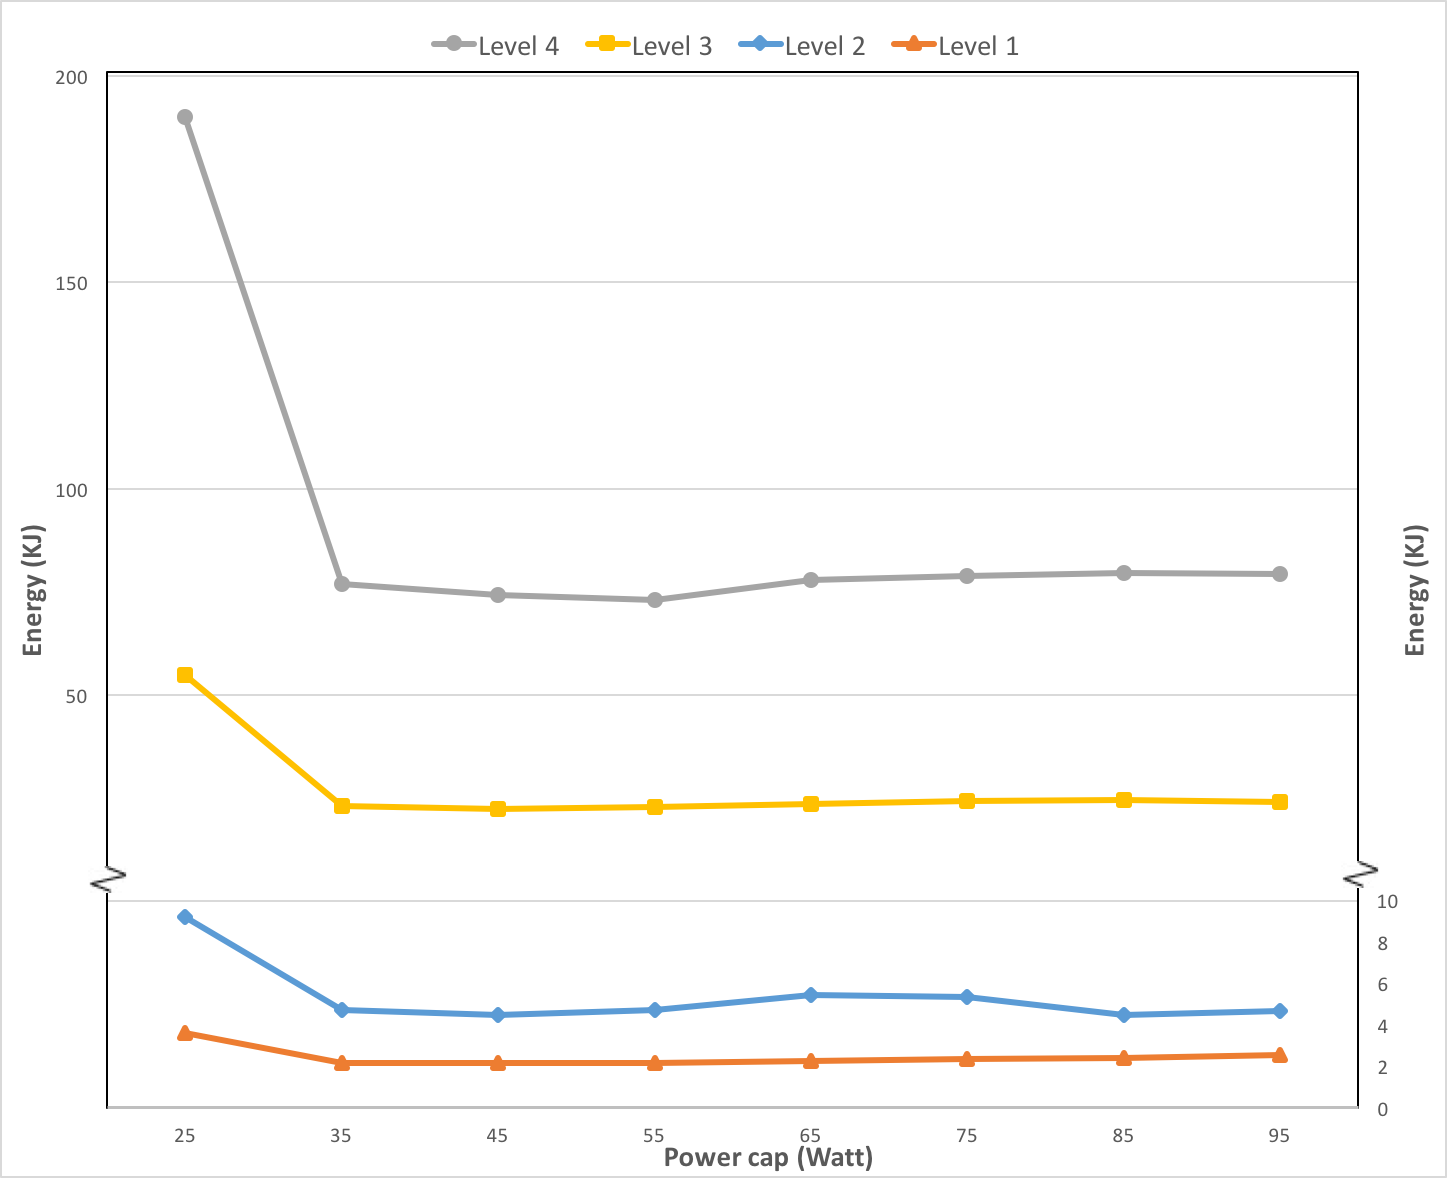
\includegraphics[width=8cm]{figs/CAPER_lev1-4_power_cap_energy_edited.png}
        \caption{Relationship between different resolution of LMC and the energy consumption under different power capping levels}
        \label{fig:RAPLpowercappower}
\end{figure}

\noindent
%\textbf{Discussion}

Figure presents the energy consumption result of executing level 1 to level 4 LMC program on certain number of cores under different power capping configurations. Those curves have the same pattern that sharply decreasing from 25 to 35 and becoming flat between 65 and 95. The lowest energy consumption is appearing when CPU power was capped to 45W to 55W. This can be explaining from execution data that without any CPU power capping, LMC program will boots CPU to 65W to 75W during execution whatever executing on how many cores. This also can be seem from the flat curve on segment 65W to 95W on each chart. Therefore, the advantage of power capping is working when CPU power down below 65W, and optimize between 45W to 55W. 



\subsubsection{Evaluation of power budget acquisition through power capping and resolution degradation}
The previous experiments have characterized the behavior of LMC. It can be concluded that the execution time will increase as the level of refinement/resolution increases or CPU power is capped down. Also, the energy consumption trend for different power caps and refinement levels is shown in Figure \ref{fig:Energy_consumption_trend}. The energy consumption presents the same trend as the execution time, i.e., LMC will consume more energy as the levels of refinement/resolution increase or capping down CPU power. The question here is how to use this characterization to create available power budget. We propose to combine these two factors, adjusting resolution and applying appropriate power capping, to get available power budget for running other tasks (e.g., checkpointing). 


\textbf{Configuration}
\begin{table}[H]
\begin{center}
\begin{tabular}{|l|l|}
	\hline
	\textbf{Parameter} & \textbf{Value}\\ \hline
    Platform & CAPER cluster\\ 		\hline
    Number of cores & 64 cores\\
	\hline
	Resolution & level 3 2 1\\
    \hline
    Time step & 10\\
    \hline
    Time unit & Second\\
    \hline
    Power measurement & RAPL meter\\
    \hline
    Power cap & RAPL\\
    \hline
\end{tabular}
\end{center}
\caption{Configuration for experiment of getting available power budget through power capping and resolution degradation
}
\label{table:table_tradeoff}
\end{table}



\begin{figure}[H]
	\centering
    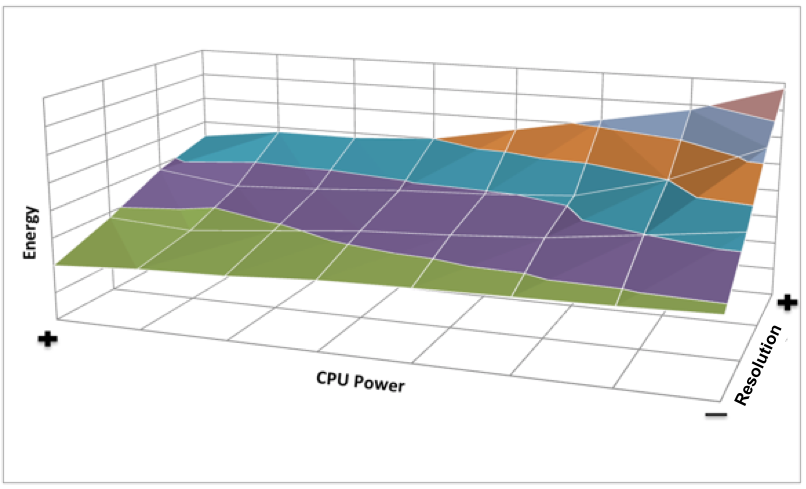
\includegraphics[width=8cm]{figs/Energy_consumption_trend.png}
        \caption{Energy consumption trend for different power caps and refinement levels}
        \label{fig:Energy_consumption_trend}
\end{figure}

\begin{figure}[H]
	\centering
    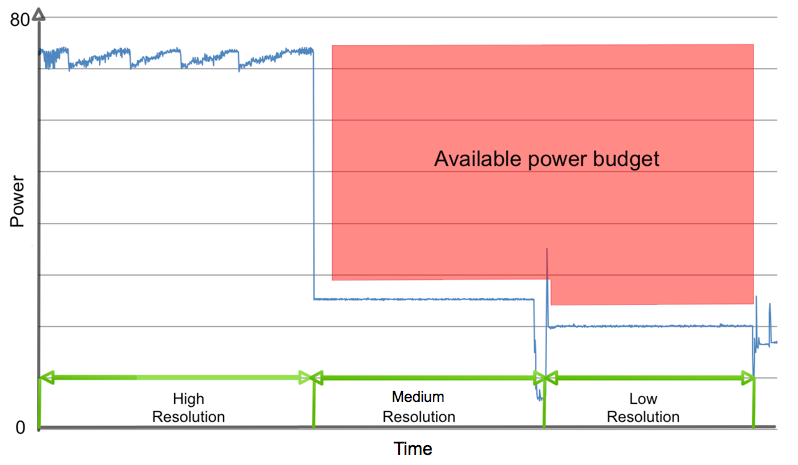
\includegraphics[width=8cm]{figs/Available_power_budget.png}
        \caption{Available power budget from applying resolution degradation and appropriate power capping}
        \label{fig:Available_power_budget}
\end{figure}


In previous Figure \ref{figs:LMCruntime}, we measured the power consumption of running LMC with different resolution. It shows that the execution time decreases when decreasing the resolution. Therefore, we apply appropriate power capping to the medium and low resolution execution to make their execution equal the execution time in highest resolution. As shown in Figure \ref{fig:Available_power_budget}, the red region is the available power budget extracted from the total power budget. 



\subsubsection{Evaluation of power budget management}
We have tested the impact of power capping and level of refinement of LMC on the performance and energy consumption. We also observed the potential power saving from degrading resolution and implementing power capping. The goal of this experiment is being able to use power budgets opportunistically for running other tasks. In the experiment, we propose to use this power budget to do  checkpointing, which will increase the resilience and make the LMC program running more reliably. 

In this experiment, we are proposing to degrade LMC resolution and cap its running power, then use this power budget to do check pointing. However, there are some limitations due to the code characteristics: (i) we can not separate the checkpoint function from simulation program, and (ii) we can not dynamically control LMC resolution. 

%\textbf{Methodology}\\
To address these two issues, we use two LMC executions running alternatively on two set of nodes to emulate one execution dynamically adjusting resolution and doing checkpoint. Each set of nodes contains three nodes for execution. When the first execution start doing checkpoint then the second set start another execution with lower resolution. We focus on system level power consumption. 

We implement this using a flag to coordinate these two LMC executions. We've recompiled the first LMC set program to let it write flag when it start to do checkpoint, and the second LMC set keeps reading the flag to start running when the flag turn to be true. As shown in Figure \ref{fig:lev3withoutpowercap}, when the blue curve is the first instance (set 1) of LMC finishes its execution, it triggers the second instance (set 2), which is the orange curve. Once the second instance is completed the first one is triggered again and so on. By doing this, we can emulate a single LMC execution running and dynamically change the resolution while giving the available power budget for doing checkpoint.



\textbf{Configuration}
\begin{table}[H]
\begin{center}
\begin{tabular}{|l|l|}
	\hline
	\textbf{Parameter} & \textbf{Value}\\ \hline
    Platform & CAPER cluster\\ 		\hline
    Number of cores & 64 cores\\
	\hline
    Resolution & level 4 3\\
    \hline
    Time step & 10\\
    \hline
    Time unit & Second\\
    \hline
    Power measurement object & 3 nodes processors\\
    \hline
    Power cap & RAPL\\
    \hline
\end{tabular}
\end{center}
\caption{Configuration for experiment of exploring the power-performance tradeoffs 
}
\label{table:table_tradeoff}
\end{table}



\begin{figure}[H]
	\centering
    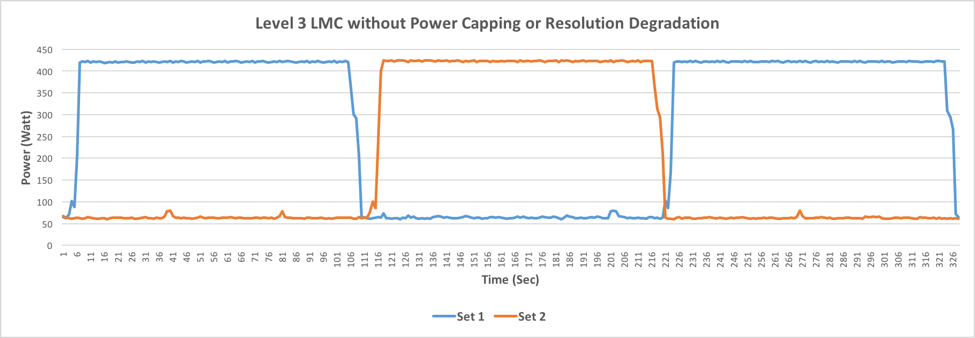
\includegraphics[width=8cm]{figs/lev3withoutpowercap.png}
        \caption{Level 3 LMC power consumption without power capping or resolution degradation}
        \label{fig:lev3withoutpowercap}
\end{figure}


\begin{figure}[H]
	\centering
    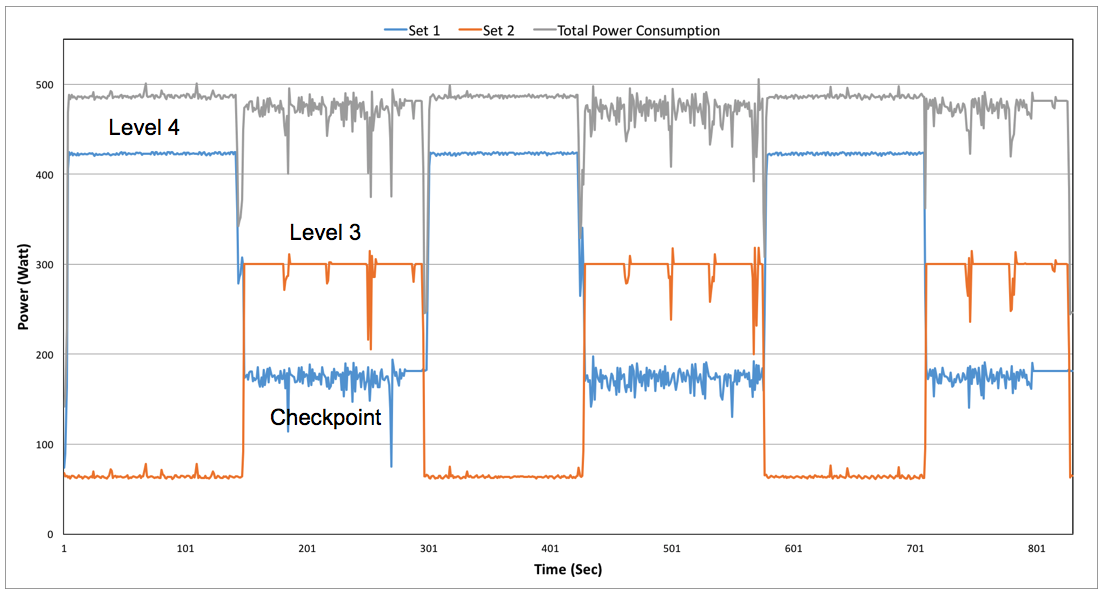
\includegraphics[width=8cm]{figs/LMCtradeoff.png}
        \caption{Level 4 LMC power consumption with power capping or resolution degradation}
        \label{fig:LMCtradeoff}
\end{figure}

In Figure \ref{fig:LMCtradeoff}, the blue curve is the set 1 running the high resolution LMC (level 4). Once it starts doing checkpointing, the set 2 (in orange curve) is triggered to run LMC at level 3. Configuring power capping appropriately, the total power consumption, which is shown in gray curve on the top, is kept constant. This means we successfully constraint the power budget of LMC to perform other tasks (i.e., checkpointing).


\section{Conclusion and Future work}
\label{Section:conclution}

In this work, we  have focused on studying the properties and exploring the performance, quality and power/energy tradeoffs of Low-Mach-Number Combustion (LMC) application which is based Adaptive Mesh Refinement (AMR) algorithm. The key contributions of this work are (1) we present an empirical evaluation of different configurations of application that gives insights into the energy-performance-quality tradeoff for this work, (2) we provided a comprehensive study of this LMC simulation performance, power and energy behavior, and (3) we propose a power-performance-quality tradeoff for this application, which can be used to better schedule power budgets across HPC systems.

Our current work investigates how to leverage these insights to implement a runtime to manage power budgets dynamically. Moreover, instead of trading-off with resolution, we also plan to explore the possibility of managing resources dynamically (e.g., cores) to manage power budgets. Future work also includes the management and scheduling of power budgets at whole system scale for assigning power budgets to other applications, not necessarily to the LMC workflow.


% An example of a floating figure using the graphicx package.
% Note that \label must occur AFTER (or within) \caption.
% For figures, \caption should occur after the \includegraphics.
% Note that IEEEtran v1.7 and later has special internal code that
% is designed to preserve the operation of \label within \caption
% even when the captionsoff option is in effect. However, because
% of issues like this, it may be the safest practice to put all your
% \label just after \caption rather than within \caption{}.
%
% Reminder: the "draftcls" or "draftclsnofoot", not "draft", class
% option should be used if it is desired that the figures are to be
% displayed while in draft mode.
%
%\begin{figure}[!t]
%\centering
%\includegraphics[width=2.5in]{myfigure}
% where an .eps filename suffix will be assumed under latex, 
% and a .pdf suffix will be assumed for pdflatex; or what has been declared
% via \DeclareGraphicsExtensions.
%\caption{Simulation Results}
%\label{fig_sim}
%\end{figure}

% Note that IEEE typically puts floats only at the top, even when this
% results in a large percentage of a column being occupied by floats.


% An example of a double column floating figure using two subfigures.
% (The subfig.sty package must be loaded for this to work.)
% The subfigure \label commands are set within each subfloat command, the
% \label for the overall figure must come after \caption.
% \hfil must be used as a separator to get equal spacing.
% The subfigure.sty package works much the same way, except \subfigure is
% used instead of \subfloat.
%
%\begin{figure*}[!t]
%\centerline{\subfloat[Case I]\includegraphics[width=2.5in]{subfigcase1}%
%\label{fig_first_case}}
%\hfil
%\subfloat[Case II]{\includegraphics[width=2.5in]{subfigcase2}%
%\label{fig_second_case}}}
%\caption{Simulation results}
%\label{fig_sim}
%\end{figure*}
%
% Note that often IEEE papers with subfigures do not employ subfigure
% captions (using the optional argument to \subfloat), but instead will
% reference/describe all of them (a), (b), etc., within the main caption.


% An example of a floating table. Note that, for IEEE style tables, the 
% \caption command should come BEFORE the table. Table text will default to
% \footnotesize as IEEE normally uses this smaller font for tables.
% The \label must come after \caption as always.
%
%\begin{table}[!t]
%% increase table row spacing, adjust to taste
%\renewcommand{\arraystretch}{1.3}
% if using array.sty, it might be a good idea to tweak the value of
% \extrarowheight as needed to properly center the text within the cells
%\caption{An Example of a Table}
%\label{table_example}
%\centering
%% Some packages, such as MDW tools, offer better commands for making tables
%% than the plain LaTeX2e tabular which is used here.
%\begin{tabular}{|c||c|}
%\hline
%One & Two\\
%\hline
%Three & Four\\
%\hline
%\end{tabular}/Users/qybo123/Dropbox/power capping porject/paper/2017CCGrid/approach.tex
%\end{table}


% Note that IEEE does not put floats in the very first column - or typically
% anywhere on the first page for that matter. Also, in-text middle ("here")
% positioning is not used. Most IEEE journals/conferences use top floats
% exclusively. Note that, LaTeX2e, unlike IEEE journals/conferences, places
% footnotes above bottom floats. This can be corrected via the \fnbelowfloat
% command of the stfloats package.



% use section* for acknowledgement
\section*{Acknowledgment}
The authors would like to thank...
more thanks here

% trigger a \newpage just before the given reference
% number - used to balance the columns on the last page
% adjust value as needed - may need to be readjusted if
% the document is modified later
%\IEEEtriggeratref{8}
% The "triggered" command can be changed if desired:
%\IEEEtriggercmd{\enlargethispage{-5in}}

% references section

% can use a bibliography generated by BibTeX as a .bbl file
% BibTeX documentation can be easily obtained at:
% http://www.ctan.org/tex-archive/biblio/bibtex/contrib/doc/
% The IEEEtran BibTeX style support page is at:
% http://www.michaelshell.org/tex/ieeetran/bibtex/
%\bibliographystyle{IEEEtran}
% argument is your BibTeX string definitions and bibliography database(s)
%\bibliography{IEEEabrv,../bib/paper}
%
% <OR> manually copy in the resultant .bbl file
% set second argument of \begin to the number of references
% (used to reserve space for the reference number labels box)
%\begin{thebibliography}{1}

%\bibitem{IEEEhowto:kopka}
%H.~Kopka and P.~W. Daly, \emph{A Guide to \LaTeX}, 3rd~ed.\hskip 1em plus
 % 0.5em minus 0.4em\relax Harlow, England: Addison-Wesley, 1999.

%\end{thebibliography}


\bibliographystyle{IEEEtran}
\bibliography{references}

% that's all folks
\end{document}


